\documentclass[mathserif, aspectratio=169]{beamer}
%
%%%%%%%%%%%%%%%%%%%%%%%%%%%%%%%%%%%%%%%%%%%%%%%%%%%%%%%%%%%%%%%%%%%%%%%%
% need to split the includes to make spell checking work.
\usepackage{arev, arevmath}
\usepackage[scaled]{cabin}
\usepackage[T1]{fontenc}
\usepackage[super]{nth}
\usepackage{pifont}
\usepackage{wasysym}
\usepackage{tabularx}
\usepackage{array}
\usepackage{booktabs}
\usepackage{boldline}
\usepackage{colortbl}
%\usepackage{amsmath}
\usepackage{bm}
\usepackage{tcolorbox}
\usepackage{adjustbox}
\usepackage{minibox}
\usepackage{makecell}
\usepackage{adjustbox}
\usepackage{textcomp}
\usepackage[absolute,overlay]{textpos}
\setlength{\TPHorizModule}{1mm}%
\setlength{\TPVertModule}{1mm}%
\tcbuselibrary{skins}

\makeatletter
\newcommand{\antsize}{\@setfontsize{\antsize}{4pt}{4pt}}
\makeatother
\newcommand{\at}{\makeatletter @\makeatother}

\newcommand{\cmark}{\ding{51}}%
\newcommand{\bottomline}[1]{\vskip0pt plus 1fill{\alert{#1}\phantom{g}\vskip 1.0mm}}

\newcommand{\Quote}[2]{%
	\begin{center} 
		\begin{minipage}{0.7\textwidth} 
			\hrule
			\vskip 3mm
			\emph{{\color{ICTPblue} ``#1''}
			
			~~~~ {\color{ICTPorange} --- #2}}
			\vskip 3mm
			\hrule
			\vskip 2mm
		\end{minipage}
	\end{center}}


\mode<presentation>%
{
	\usetheme{default}
	%\usetheme[width=2.5cm]{PaloAlto}
	\usecolortheme{dove}
	\useoutertheme{infolines}
	% oder auch nicht

	% ICTP Colors
	\definecolor{ICTPblue}{RGB}{37,86,162} % 0x255682
	\definecolor{ICTPorange}{RGB}{255,130,0} % 0xff8200
	\definecolor{ICTPgreen}{RGB}{0,100,0}
	\definecolor{ICTPdark}{RGB}{80,80,80} % 0x505050
	\definecolor{ICTPlight}{RGB}{120,120,120}
	\definecolor{ICTPbrown}{RGB}{178,91,0}

	\definecolor{codebg}{rgb}{0.95,0.95,0.95}

	% Color theme
	\setbeamercolor{alerted text}{fg=ICTPorange}
	\setbeamercolor{frametitle}{fg=ICTPblue}
	\setbeamercolor{title}{fg=ICTPblue}
	\setbeamercolor{subtitle}{fg=ICTPorange}
	\setbeamercolor{normal text}{fg=ICTPdark}
	\setbeamercolor{author in foot}{fg=ICTPblue}
	\setbeamercolor{item}{fg=ICTPblue}
	\setbeamercolor{footline}{fg=ICTPblue}
	%\setbeamercolor{item projected}{bg=ICTPorange}
	%\setbeamercolor{item projected}{fg=white}

	\setbeamertemplate{headline}
	{}
	\setbeamertemplate{frametitle}
	{
		%\textbf{{\insertframetitle\phantom{g}}}\\
		%\textbf{\insertframetitle\phantom{g}}\\
		\textbf{\underline{\insertframetitle\phantom{g}}}\\
		%\textbf{\underline{\insertframetitle}}\\
		\vskip 1.0mm
		%{\color{UOLgold}\hrule height 2pt}
		%\par
	}
	\addtobeamertemplate{frametitle}{}{\vspace{-1em}}
	\setbeamertemplate{footline}{
		{%
			\textbf{ \hskip 3.0mm\insertshorttitle\phantom{.}---\phantom{.}\insertshortinstitute\hfill\insertframenumber\,/\,\inserttotalframenumber\hskip 3.0mm} 
		}
	}

	\setbeamertemplate{navigation symbols}{}%remove navigation symbols
	\setbeamertemplate{itemize items}[circle]
	\setbeamertemplate{enumerate items}[fg=ICTPblue]
	\setbeamercolor{itemize items}{fg=ICTPblue}
	\setbeamercolor{sidebar}{bg=ICTPblue}
	\setbeamercolor{title in sidebar}{fg=ICTPorange}
	\setbeamercolor{author in sidebar}{fg=ICTPorange}
	\setbeamercolor{section in sidebar}{fg=ICTPorange}
}

%\input{tikz/common-styles}

\usepackage{graphicx}
\usepackage[latin1]{inputenc}

\graphicspath{{../figs/}{../figs/common/}{../figs/islr/}}

\title[Statistical Learning] % (optional, nur bei langen Titeln n�tig)
{\textbf{Introduction to Statistical Learning\\ {\it with applications in Python}}\\%
		\href{www.statlearning.com}%
		{\tiny\it Based on ``Introduction to Statistical Learning, with applications in R'' by Gareth James, Daniela Witten, Trevor Hastie, Robert Tibishirani}\vspace{2em}}
		\vspace{-2.5cm}{}


		\author{\href{mailto:?to=Kurt Rinnert <kurt.rinnert@cern.ch>&subject=PWF Statistical Learning}{Kurt Rinnert}}

\institute[{\href{https://www.ictp.it/physics-without-frontiers.aspx}{Physics Without Frontiers} --- \href{https://www.ictp.it/}{ICTP}}] % (optional)
{\color{ICTPblue}\bfseries \href{https://www.ictp.it/physics-without-frontiers.aspx}{Physics Without Frontiers}\\\vspace{1mm}%
\href{https://www.ictp.it/}{
\includegraphics[width=0.20\textwidth]{common/ICTP-logo-full-trans.png}}\\%
\href{https://www.liverpool.ac.uk/physics/}{
\includegraphics[width=0.2\textwidth]{common/uol_logo.png}}}

\date{}

\titlegraphic{
	\texorpdfstring{\vspace{-2.8cm}}{}
	 \begin{minipage}[b][1.3cm][b]{0.26\textwidth}\color{ICTPlight}\antsize
		Copyright \textcopyright~2019\\
		\href{mailto:?to=Kurt Rinnert <kurt.rinnert@cern.ch>&subject=PWF Statistical Learning}{Kurt Rinnert <kurt.rinnert{\tt @}cern.ch>},
		\href{mailto:?to=Kate Shaw <kshaw@ictp.it>&subject=PWF Statistical Learning}{Kate Shaw <kshaw{\tt @}ictp.it>}\\
		Copying and distribution of this file, with or without modification,
		are permitted in any medium without royalty provided the copyright
		notice and this notice are preserved.  This file is offered as-is,
		without any warranty.


		Some of the figures in this presentation are taken from ``An Introduction to
		Statistical Learning, with applications in R''  (Springer, 2013) with
		permission from the authors: G. James, D. Witten,  T. Hastie and R. Tibshirani 
	 \end{minipage}\hspace{10cm}
}


\addtocounter{framenumber}{-1}

% nicer table row separation
\renewcommand{\arraystretch}{1.2}

% color boxes
\newcommand{\tabboxset}{\tcbset{enhanced, nobeforeafter, boxrule=0pt, boxsep=0pt, colback=codebg, colframe=codebg, coltext=ICTPdark, rounded corners, arc=4pt, fonttitle={\bfseries\tiny}}}
\newcommand{\codeboxset}{\tcbset{enhanced, nobeforeafter, boxrule=0pt, boxsep=0pt, colback=codebg, colframe=codebg, coltext=ICTPdark, rounded corners, arc=4pt, fonttitle={\bfseries\tiny}}}

\newcommand{\orange}{\color{ICTPorange}}
\newcommand{\blue}{\color{ICTPblue}}
\newcommand{\dark}{\color{ICTPdark}}
\newcommand{\R}{\mathbb{R}}
\newcommand{\dat}[1]{{\footnotesize\tt\orange #1}}
\newcommand{\e}[1]{\emph{#1}}
\newcommand{\bh}{\hat{\beta}}
\newcommand{\h}{\hat}

\makeatletter
\newcommand{\includegraphicsdpi}[3]{%
	\pdfimageresolution=#1%
	\includegraphics[#2]{#3}%
	\pdfimageresolution=72%
}

\newenvironment{blurb}%
	{\begin{center}\begin{minipage}{0.6\textwidth}\footnotesize}
	{\end{minipage}\end{center}}

\newenvironment{cpage}%
	{\begin{center}\begin{minipage}{0.75\textwidth}}
	{\end{minipage}\end{center}}

\newenvironment{popblock}[2]%
	{\begin{center}\begin{minipage}{#1}\footnotesize
		\begin{tcolorbox}[colframe=codebg, colback=white, colupper=ICTPdark, title={\normalsize\bfseries\blue #2}]}
	{\end{tcolorbox}\end{minipage}\end{center}}
\makeatother

\subtitle{\bfseries%
  {Linear Regression, Part 2}\\%
  {\tiny\it multiple linear regression, qualitative predictors, interaction \& non-linear terms, leverage and other considerations}\\%
}
\begin{document}
\frame[plain]{
	\vskip 1.0mm
	\titlepage
	\vskip 1.0mm
}


\begin{frame}{Abstract}

	\begin{blurb}
		Linear models are an important topic in statistical learning.  

		The true relationships between predictors and responses are rarely linear.
		But linear models often provide reasonable approximation. They provide
		high interpretability and have low variance, mitigating the risk of over-fitting.
		Linear models can be extended to include (some) non-linear relationships. 

		Linear models also provide an excellent baseline to compare other models against: if 
		our sophisticated model does not do much better than a linear model we might consider
		trading some bias for lower variance.
	\end{blurb}
\end{frame}

\begin{frame}{Overview}
	\begin{itemize}
		\item Linear models with multiple predictors.
		\item Qualitative predictors.
		\item Extensions to the linear model.
		\item Leverage and other considerations.
	\end{itemize}
	\bottomline{This will require some mathematics.}
\end{frame}

\begin{frame}{The Scenario}
	\begin{itemize}
		\item We look at the \dat{Advertising} data set again.
		\item Previously, we only used the \dat{TV} predictor to predict \dat{sales}.
		\item The data set provides two more predictors, \dat{radio} and \dat{newspaper}.
		\item We are now interested in using all available information in the data set.
		\item We can think of two ways of doing that:
			\begin{cpage}
				\begin{enumerate}
					\item Perform simple linear regression on the predictors separately.
					\item Somehow combine all predictors.
				\end{enumerate}
			\end{cpage}
	\end{itemize}
	\bottomline{As you might guess, option two is more interesting, but let's look at option one first.}
\end{frame}

\begin{frame}{Separate Simple Linear Regression}
	\begin{center}
		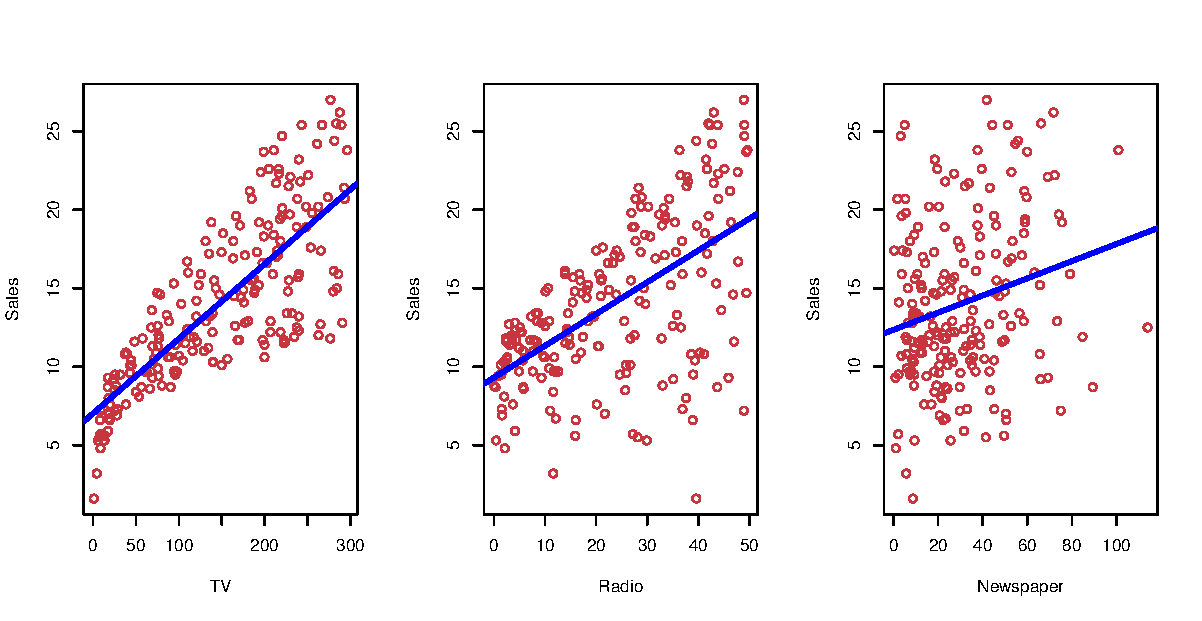
\includegraphics[width=0.7\textwidth]{2_1}
	\end{center}
	\bottomline{Separate simple linear regression looks promising on this data set.}
\end{frame}

\begin{frame}{Separate Simple Linear Regression}
	\begin{popblock}{0.7\textwidth}{Regression of \dat{sales} onto \dat{radio}}
		\begin{tabular}[h]{lrrrr}
			{} & {\blue Coefficient} & {\blue Std. Error} & {\blue $t$-statistic} & {\blue $p$-value} \\
			\dat{Intercept} & 9.312 & 0.563 & 16.54 & $< 0.0001$ \\
			\dat{radio} & 0.203 & 0.020 & 9.92 & $< 0.0001$ \\
		\end{tabular}
	\end{popblock}
	\begin{popblock}{0.7\textwidth}{Regression of \dat{sales} onto \dat{newspaper}}
		\begin{tabular}[h]{lrrrr}
			{} & {\blue Coefficient} & {\blue Std. Error} & {\blue $t$-statistic} & {\blue $p$-value} \\
			\dat{Intercept} & 12.351 & 0.621 & 19.88 & $< 0.0001$ \\
			\dat{newspaper} & 0.055 & 0.017 & 3.30 & $ 0.00115$ \\
		\end{tabular}
	\end{popblock}
	\bottomline{All the separate regressions look reasonable.}
\end{frame}

\begin{frame}{Separate Simple Linear Regression}
	\begin{itemize}
		\item This is not entirely satisfactory for several reasons.
		\item It is unclear how could predict a single value of \dat{sales} from
			the separate models.
		\item Each of the separate models ignores the other variables.
		\item This is problematic if there are correlations between the predictors.
	\end{itemize}
	\bottomline{A better approach is to use multiple predictors simultaneously.}
\end{frame}


\begin{frame}{Multiple Simple Linear Regression}
	\begin{itemize}
		\item \e{Multiple linear regression} uses multiple predictors.
		\item Each predictor has its own slope coefficient.
		\item For $p$ predictors the model takes the form
			\[ Y = \beta_0 + \beta_1 X_1 + \beta_2 X_2 + \dots + \beta_p X_p + \epsilon \]
			where the $\beta_j$ are interpreted as the average effect $X_j$ has on $Y$ while\\
			\e{holding all other predictors constant}.
		\item For example:
			\[ \text{\dat{sales}} = \beta_0
				+ \beta_1\times\text{\dat{TV}}
				+ \beta_2\times\text{\dat{radio}}
				+ \beta_3\times\text{\dat{newspaper}}
				+ \epsilon
			\]
	\end{itemize}
	\bottomline{Now we have one model using all the information.}
\end{frame}

\begin{frame}{Example: Two Predictors}
	\begin{center}
		\vspace{-5mm}
		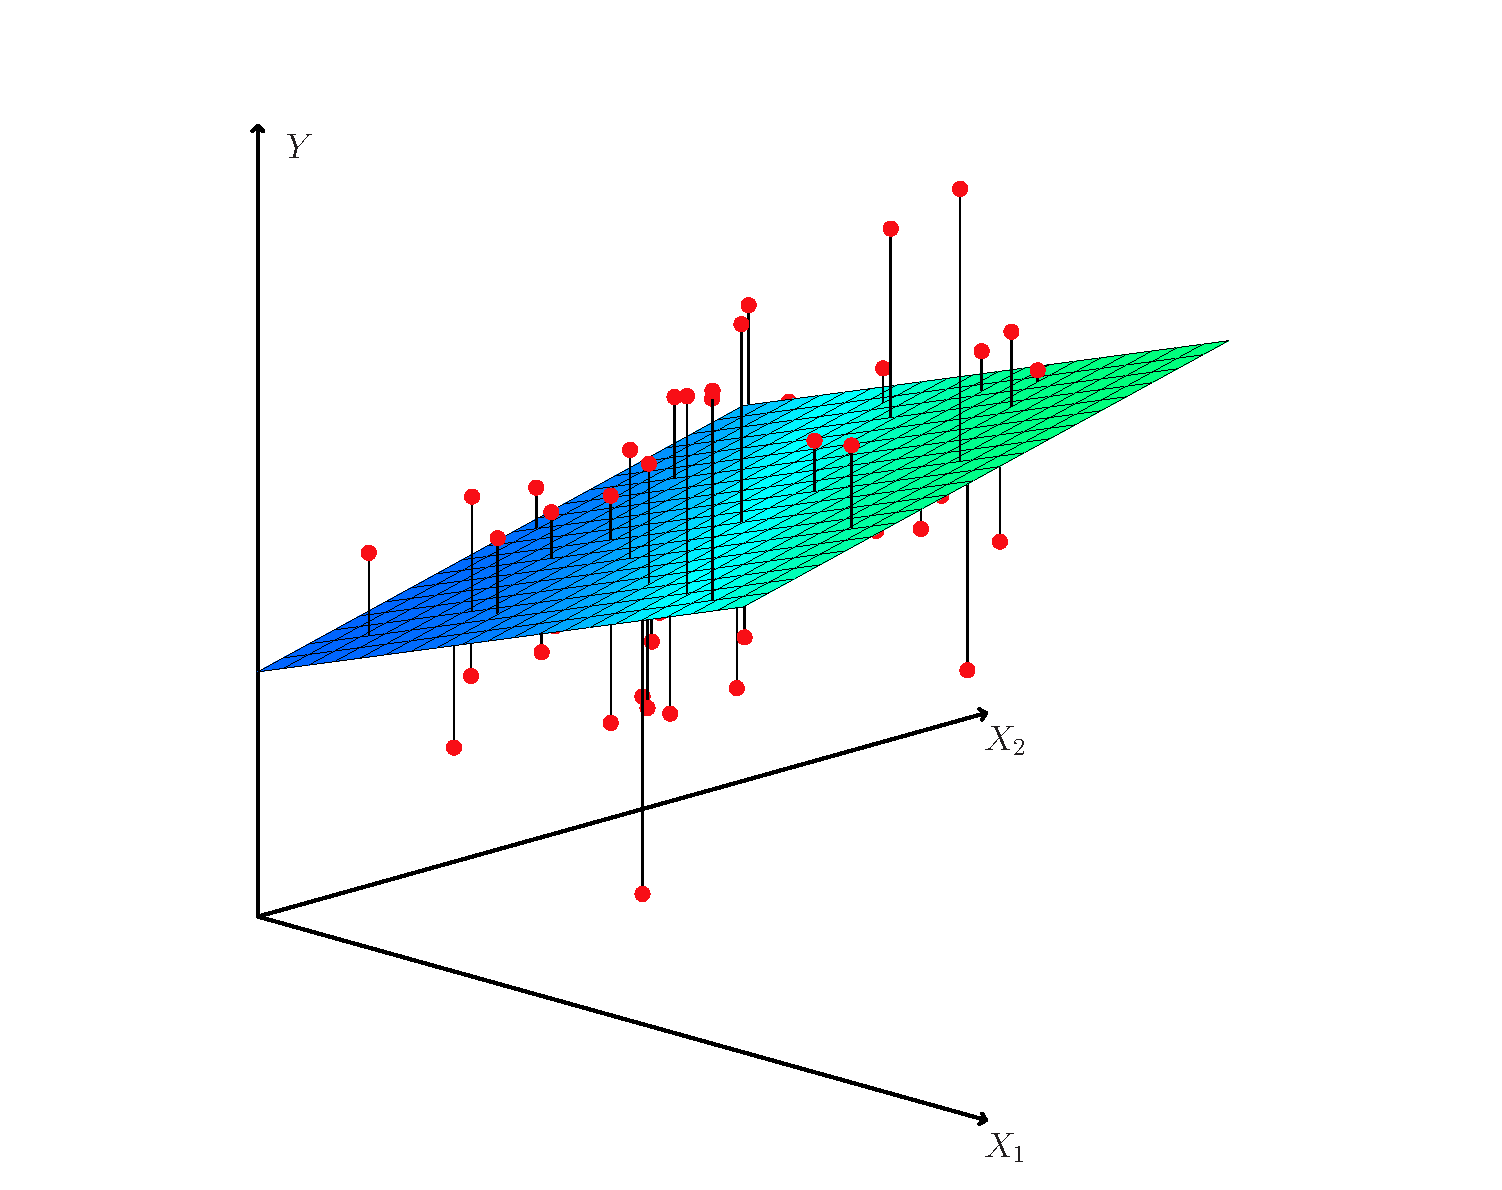
\includegraphics[width=0.5\textwidth]{3_4}

		\vspace{-8mm}
		\[ Y = \beta_0 + \beta_1 X_1 + \beta_2 X_2 + \epsilon \]
	\end{center}
	\bl{In general, the result is a \e{hyperplane}.}
\end{frame}

\begin{frame}{Estimating the Regression Coefficients}
	\begin{itemize}
		\item As in simple linear regression we want to make predictions using
			estimated parameters:
			\[ \h{y} = \bh_0 + \bh_1 x_1 + \bh_2 x_2 + \dots + \bh_p x_p \]
		\item We choose the coefficients $\bh_0, \bh_1, \bh_2, \dots, \bh_p$
			to minimise the sum of squared residuals:
			\begin{align*}
				\text{RSS} &= \sum_{i=1}^n (y_i - \hat{y}_i)^2 \\
				{} &= \sum_{i=1}^{n} (y_i - \bh_0 - \bh_1 x_1 - \bh_2 x_2 - \dots - \bh_p x_p)^2
			\end{align*}
	\end{itemize}
	\bl{Deriving the solution involves some matrix manipulations.}
\end{frame}
\end{document}
